\documentclass{article}

\usepackage{enumitem}
\usepackage[a4paper, hmargin=3cm, tmargin=2cm]{geometry}
\usepackage{fontspec}
\usepackage{minted}
\usepackage[dvipsnames]{xcolor}
\usepackage{setspace}

\usepackage{tikz}
\usetikzlibrary{backgrounds}


\setmainfont{URW Bookman}
\setmonofont{Iosevka}

\title{\Large \textbf{Computação Concorrente}
	\vspace{0.5em}\\
	\large Lista 1
}

\author{Igor de Araujo Vilhalba}
\date{12/08/2021}

\setlength{\parskip}{1em}

\setminted[c]{ %
    linenos=true,
    autogobble=true,
	bgcolor=pink
}

\newcommand{\Tz}{\textbf{T0}}
\newcommand{\Tu}{\textbf{T1}}
\newcommand{\Td}{\textbf{T2}}
\newcommand{\Tt}{\textbf{T3}}

\newcommand{\TL}[2]{\textbf{(#1)}$_{T#2}$}

\begin{document}

\maketitle

\section*{Questão 1}

\begin{enumerate}[label=\textbf{\alph*)}]
	% a)
	\item Um programa concorrente é caracterizado pela presença de fluxos de execução,
		enquanto um programa sequencial possui apenas uma. Podemos pensar em fluxos
		de execução como uma sequência de instruções. Se um programa é concorrente,
		há mais de uma sequência de instruções que serão tratadas independentemente.\\
		É importante notar que a concorrência não implica na execução simultânea de
		mais de um fluxo de execução (\emph{paralelismo}).
	\item Para problemas que podem ser divididos em subtarefas que independem umas das
		outras. Isso é, podemos dividir o problema em múltiplos fluxos de execução
		onde a execução de um não depende do término de outro. Se houvesse essa
		dependência, o modelo seria sequencial, não concorrente.
	\item O limite teórico para o ganho de performance (aceleração), de acordo com
		a \textbf{lei de Amdahl} é
		\begin{center}
			$$
			Acel = \frac{T_s + T_P(1)}{T_s+T_P(P)}
			$$
			onde $T_P(1)$ é o tempo de execução da parte concorrente do programa
			em um único fluxo, $T_s$ é a parte estritamente sequencial do programa
			(não é dividida entre as threads) e $T_P(P)$ é a parte concorrente com
			o uso de $P$ processadores (ou núcleos).
		\end{center}

		{\footnotesize \textbf{Obs.:} Para fazermos os cálculos, vamos substituir a palavra
		\emph{concorrente} por \emph{paralela}, já que é com base nisso que a lei de Amdahl
		nos dá a aceleração.}

		Como nesse caso não há duas tarefas que executam sequencialmente, elas que vão compor
		$T_s$. Digamos que cada tarefa consuma o tempo $T$. Disso tiramos que $T_s = 2T$ (já que
		são \textbf{duas} tarefas que gastam tempo $T$).


		Como são três tarefas que serão executadas concorrentemente e cada tarefa gasta o tempo $T$,
		temos que essas três tarefas quando executadas sequencialmente (por um único processador,
		em outras palavras) gastam $3T$. Ou seja, $T_P(1) = 3T$. Temos, também que essas três tarefas
		quando executadas por três processadores (paralelamente) gastam o tempo $T_P(P) = 3T/3 = T$.
		Agora basta substituirmos na equação.

		\begin{center}

		\tikzstyle{background rectangle}=[thin,draw=black]
		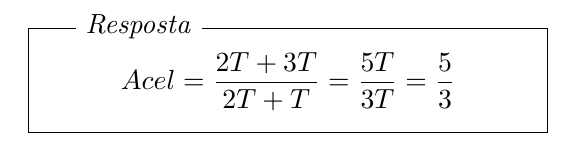
\begin{tikzpicture}[show background rectangle]
		\node[align=justify, text width=0.5\textwidth]{
			$$
			Acel = \frac{2T + 3T}{2T + T} = \frac{5T}{3T} = \frac{5}{3}
			$$
		};

		\node[xshift=3ex, yshift=-0.7ex, overlay, fill=white, draw=white, above 
		right] at (current bounding box.north west) {
		\textit{Resposta}
		};

\end{tikzpicture}
		\end{center}

	\item A \emph{seção crítica} é uma porção do código que acessa algum recurso
		compartilhado que não pode ser acessado por mais de um fluxo ao mesmo tempo.
	\item É uma técnica de sincronização que consiste em ``\emph{travar}'' a seção crítica
		das demais threads caso alguma delas já tenha entrado nela.\\
		Essa técnica funciona com uma ``trava'' (\emph{mutex lock}). Quando uma thread
		chega na seção crítica, antes de executá-la, verifica se ela está destravada
		(se a trava está ``desativada'' ou, em outras palavras, nenhuma outra thread
		possui a trava). Se a seção estiver travada, a thread é interrompida, e o controle
		é passado para outra qualquer (isso fica a cargo do sistema operacional), já que
		ela não pode prosseguir com a execução.\\
		Caso a seção crítica esteja destravada, essa thread passa a possuir a trava, fazendo
		com que as demais não possam entrar na seção crítica enquanto esta thread não a soltar.
\end{enumerate}

\section*{Questão 2}

Como uma função que é chamada por \texttt{pthread\_create()} recebe como argumento apenas um ponteiro,
precisamos definir uma \emph{struct} para passar os argumentos para ela. A chamaremos de \texttt{args\_t}.\\
Sua declaração é como segue:

\begin{minted}{c}
typedef struct {
	int id; // identificador da thread
	int nt; // numero de threads
	int n; // quantidade de termos - 1
	double res; // escreveremos o resultado aqui
} args_t;
\end{minted}

Antes de falar sobre a estratégia utilizada, vamos reescrever o somatório de $\pi$ da seguinte forma:
\begin{center}
	$$
	\pi = \sum_{i=0}^n{(-1)^ia_i} 
	$$
	onde $a_i = \frac{4}{2i+1}$
\end{center}

A estratégia utilizada será calcular os itens intercalados. Cada thread começará calculando o termo
$a_{id+nt*k}$, para $k=0,1,...,m$ e $nt*m \le n$.

Escolhi essa estratégia pelo seguinte motivo: se o somatório fosse particionado em $nt$ partes,
a thread que ficasse encarregada de calcular os termos iniciais do somatório acabaria tendo um
resultado numérico bem maior que o da que ficasse com os termos próximos de $n$, visto que conforme
$i$ aumenta, $a_i$ se aproxima de zero. Isso pode ter consequências sobre a precisão da
operação de soma em ponto flutuante. Por esse motivo, cada thread calculará tanto os termos iniciais
(mais próximos de 1) quanto os finais (mais próximos de 0). Assim, cada uma das threads retornará números
com ordens de grandeza iguais (ou próximas).

Agora basta escrever a função.

\begin{minted}{c}
void *calcula_pi(void *arg) {
	// nao vamos liberar a memoria.
	// isso sera obrigacao de quem criou a struct
	t_args *args = (t_args *)arg;
	int id = args->id;
	int nt = args->nt;
	int n = args->n;
	double soma = 0;

	for (int i = id; i <= n; i += nt) {
		int a_i = 4 / (2*i + 1);
		if (i % 2 == 0) {
			soma += a_i;
		} else {
			soma -= a_i;
		}
	}

	args->res = soma;

	return NULL;
}
\end{minted}

Como podemos ver, o resultado está sendo retornado na própria \emph{struct} que foi passada como
argumento para a função. Fiz essa escolha para evitar usar o \texttt{malloc()} para guardar apenas
um valor. Uma alternativa possível seria retornar o valor da variável \texttt{soma} através de um
\emph{typecast}, fazendo com que se passasse pelo tipo \texttt{void *}. Entretanto, não há como garantir
que o tamanho do tipo \texttt{double} é o mesmo do tipo \texttt{void *} em todas as arquiteturas.

\section*{Questão 3}

Para simplificar, vamos desconsiderar as instruções de máquina (lê-atualiza-escreve), apenas as analizando
se necessário. Vamos olhar para cada valor e analizar se há uma sequência de linhas possível para obtar o
resultado. Para indicar a sequência de linhas executadas, com sua respectiva thread, vamos usar a notação
\textbf{(n)}$_{Tk}$, onde $n$ é a linha e $k$ é o número da thread.

\begin{itemize}
	\item \textbf{-1}\par
		Se \Tu\ executar por inteiro sem que as outras duas threads sejam executadas, $-1$ será impresso.
	\item \textbf{0}\par
		Se \Tu\ executar, mas antes de conseguir executar a linha \textbf{(5)} a linha \TL{1}{3}
		for executada (e possívelmente a thread \Td\ inteira), então quando \Tu\ voltar a executar, vai imprimir 1.
	\item \textbf{2}\par
		A sequência de linhas \TL{1}{3}--\TL{2}{3}--\TL{1}{1}--\TL{2}{1}--%
		\TL{1}{2}--\TL{3}{3} é capaz de imprimir o valor 2.
	\item \textbf{-2}\par
		Se \Tu\ e \Td\ executarem paralelamente e \TL{3}{1} estiver executanto ao mesmo tempo de \TL{1}{2},
		como vimos em aula, pode ser que \Tu\ leia o valor de x e o decremente no registrador (sem ainda escrever
		de volta na memória), enquanto \Td\ faz o mesmo. Entretanto, se \Td\ fizer a escrita antes de \Tu, \Tu\
		sobrescreverá a escrita feita por \Td.\\
		Por exemplo, após a execução de \TL{2}{1}, \texttt{x=0}. \Tu\ vai ler x e decrementar no registrador e
		\Td\ vai ler e incrementar no registrador. Se \Td\ escrever na memória primeiro, escreverá $1$ (agora \texttt{x=1}).
		Entretanto, em seguida \Tu\ escreverá na memória o valor que calculou, que é $-1$. Isso fará com que seja como se
		\TL{1}{2} nem tivesse sido executada.\\
		Agora vamos supor que \Tu\ consiga entrar no \emph{if}, já que o valor de x na memória é $-1$. Então antes de executar
		a linha \TL{5}{1}, a linha \TL{2}{2} seja executada e consiga escrever na memória. Nesse ponto, x valerá $-2$. Agora,
		quando \TL{6}{1} for executada, o programa imprimirá $-2$.
	\item \textbf{3}\par
		Vamos supor que \Tt\ cosiga executar até entrar no \emph{if}. Agora, vamos supor também que \Tu\ e \Td\ executem
		paralelamente. Se, com base no mesmo argumento do exemplo anterior, a atribuição da linha \TL{1}{2} anule a da linha
		\TL{1}{1}, e após isso alinha \TL{2}{1} execute. Se após essas operações a linha \TL{3}{3} executar, o valor 3 será
		impresso.
	\item \textbf{-3}\par
		Não é possível imprimir esse valor, pois para entrar no \emph{if} da thread \Tu (com \texttt{x=-1}), só sobrará um
		decremento possível nas outras threads. Já para entrar no \emph{if} da thread \Tt (com \texttt{x=1}), só haverá três
		decrementos possíveis nas outras threads. Ou seja, se entrar em qualquer um dos dois \emph{if}s, não será possível
		decrementar x até o valor $-3$.
	\item \textbf{4}\par
		Não é possível imprimir esse valor, pois só há 3 incrementos se juntarmos as três threads.
\end{itemize}

\section*{Questão 4}

\begin{enumerate}[label=\textbf{\alph*)}]
	\item Se \Tz\ conseguir terminar a execução da linha \textbf{(2)}, há a garantia de que conseguirá
		executar a seção crítica.
		\begin{itemize}
			\item Se perder o controle entre as linhas \textbf{(2)} e \textbf{(3)} e \Tu\ começar a
				executar, \Tu\ vai fazer \texttt{TURN=0} e não vai poder executar a seção crítica (pois
				\texttt{queroEntrar\_0} vale \emph{true}).\\
				Quando o controle voltar a \Tz, a variável \texttt{TURN} não será modificada e terá o valor
				que \Tu\ deu a ela (0) e, portanto, poderá executar a seção crítica.
			\item Se chgar na linha \textbf{(3)} antes de \Tu\ começar sua execução, o valor de
				\texttt{queroEntrar\_1} será \emph{false} e, portanto, conseguirá executar a seção crítica
				sem problemas.
		\end{itemize}
	\item
		O caso da \Tu\ começar sua execução antes de \Tz\ é análogo ao caso onde \Tz\ começa primeiro.
	\item
		Se ambas começam a execução ao mesmo tempo, podemos supor que a execução é \emph{paralela} (acontece
		em duas unidades de processamento ao mesmo tempo). Então vamos considerar que cada linha seja executada
		praticamente ao mesmo tempo. A linha \textbf{(1)} não apresenta nenhum problema. Entretanto, quando
		chegarem à linha \textbf{2} a escrita na variável \texttt{TURN} não acontecerá realmente ao mesmo tempo.
		Na prática, ou \Tz\ ou \Tu\ vai modificála por último. Essa que modificar por último será a thread que
		executará por último sua seção crítica.
	\item
		Sim. Como uma thread muda a variável \texttt{TURN} para que a vez seja da outra thread, a thread em
		questão não espera que seja ela que vai executar a seção crítica. Ela só executará ou se a veriável
		\texttt{queroEntrar\_x} (x sendo 0 ou 1) valer \emph{false} ou se a outra thread fizer
		\texttt{TURN} permitir que esta thread execute a seção crítica. Nesse caso, a outra thread não executará
		se esta thread tiver a variável \texttt{queroEntrar\_x} como \emph{true}.
\end{enumerate}

\end{document}
